\documentclass[a4paper,12pt]{article}
\usepackage{polski}
\usepackage[utf8]{inputenc}
\usepackage{graphicx}
\usepackage{fancyhdr}
\usepackage[svgnames]{xcolor}
\usepackage{float}
\usepackage{titlesec}
\usepackage{hyperref}
\usepackage{hypcap}
\usepackage{caption}
\usepackage[font={color=violet,bf},figurename=Rysunek,labelfont={it}]{caption}

\definecolor{violet}{RGB}{75,0,130}
\hypersetup{pdftex,colorlinks=true,allcolors=black}:

\setlength{\arrayrulewidth}{1mm}
\setlength{\tabcolsep}{18pt}
\renewcommand{\arraystretch}{1.5}  	
\setcounter{secnumdepth}{4}
\titleformat{\paragraph}
{\normalfont\normalsize\bfseries}{\theparagraph}{1em}{}
\titlespacing*{\paragraph}
{0pt}{3.25ex plus 1ex minus .2ex}{1.5ex plus .2ex}



\begin{document}
\begin{titlepage}
	\centering
	
\includegraphics[width=0.3\textwidth]{ki.jpg}\par\vspace{1cm}

	{\scshape\LARGE Państwowa Wyższa Szkoła Zawodowa w Tarnowie \par}
	\vspace{1cm}
	{\scshape\Large Wydział Politechniczny \par}
	\vspace{0.5cm}
	{\scshape\large Katedra Informatyki \par}
	\vspace{1cm}
	{\scshape\Large Narzędzia i środowiska programistyczne II\par}
	\vspace{1.5cm}
	{\huge\bfseries Projekt Cinema\par}
	\vspace{2cm}
	{\Large\itshape Katarzyna Łachut, Bartłomiej Majewski, Iwona Suda\par}
	\vspace{2cm}
	{\large \today\par}
\end{titlepage}							

\newpage
\pagenumbering{gobble}					
\tableofcontents 						
\newpage



\pagenumbering{arabic}					
\pagestyle{fancy}
\fancyhf{}
\fancyhead[RO]{Projekt Cinema}
\fancyhead[L]{NiSP II}
\renewcommand{\footrulewidth}{0.4pt}		
\fancyfoot[L]{\leftmark}
\fancyfoot[LE,RO]{\thepage}				


\section{Instrukcja obsługi.}				
Stworzona strona internetowa pozwala na przeglądanie dostępnych senasów, rezerwację miejsc oraz wydrukowanie biletu. 
\begin{figure}[h!] 						
\centering
  \includegraphics[width=1.0\textwidth]{stronaglownacala.png}
  \caption{Strona główna.}					
\end{figure}

Rysunek 1. przedstawia stronę główną. 
Stałymi elementami strony jest menu oraz stopka. W menu dostępna jest: strona główna, repertuar oraz cennik.
Stopka zawiera przydatne dla użytkownika linki oraz media społecznościowe, na których można znaleźć kino. \\
Pierwszym elementem na stronie jest polecany przez kino film. Po kliknięciu w przycisk  \textcolor{orange}{"Więcej"} użytkownik zostaje przeniesiony do strony z dokładnym opisem filmu. 
Poniżej tego elementu użytkownik może sprawdzić dostępne w kinie filmy, a także może sprawdzić oceny poszczególnych dzieł.

\begin{figure}[h!]
\centering
  \includegraphics[width=1.0\textwidth]{opisfilmu.png}
  \caption{Opis filmu.}
\end{figure}
Po kliknięciu wyżej wspomnianego przycisku  \textcolor{orange}{"Więcej"} pojawia się podstrona ukazana na rysunku 2. Na tej stronie użytkownik
może sprawdzić podstawowe informacje o filmie m.in. takie jak gatunek czy reżyser. Klient może również obejrzeć na niej zwiastun filmu. \\
Po kliknięciu  \textcolor{orange}{"Zarezerwuj bilet"} użytkownikowi zostanie udostępniony widok z wyglądem sali oraz z aktualnie zajętymi miejscami. 

\newpage
\begin{figure}[h!]
\centering
  \includegraphics[width=1.0\textwidth]{rezerwacjamiejsca2.png}
  \caption{Rezerwacja miejsca.}
\end{figure}
Aby zarezerwować miejsce należy uzupełnić ukazany na rysunku 3. formularz. Po uzupełnieniu danych klient musi kliknąć na interesujące go siedzenie o kolorze czarnym i zaakceptować wybór poprzez naciśnięcie przycisku \textcolor{orange}{ "Zarezerwuj"}. 


\newpage
\begin{figure}[h!]
\centering
  \includegraphics[width=0.9\textwidth]{pobraniebiletu.png}
  \caption{Przycisk do pobrania biletu.}
\end{figure}

Po zatwierdzeniu wyboru miejsc powyżej widoku sali istnieje możliwość pobrania biletu w formacie PDF.

\newpage
\begin{figure}[h!]
\centering
  \includegraphics[width=0.9\textwidth]{zajetemiejsca.png}
  \caption{Zarezerwowane miejsca.}
\end{figure}
Po odświeżeniu strony zarezerwowane wcześniej przez użytkownika miejsca mają kolor czerwony.


\newpage
\begin{figure}[h!]
\centering
  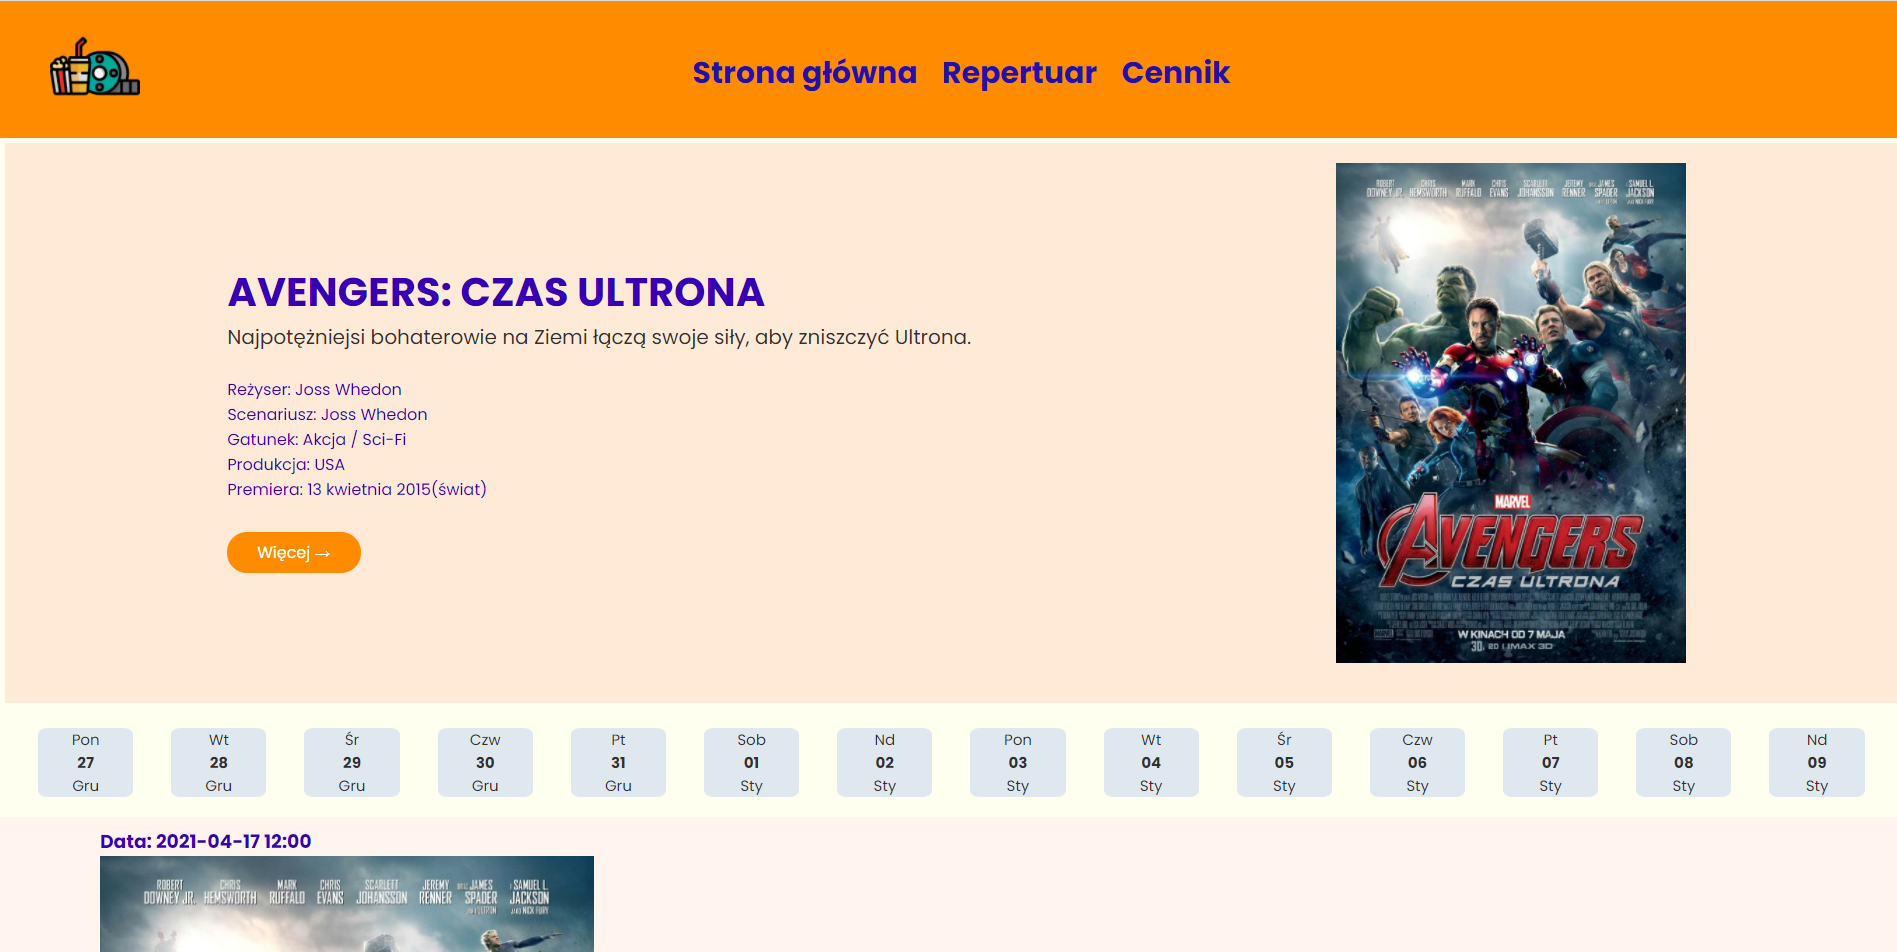
\includegraphics[width=0.6\textwidth]{repertuar.png}
  \caption{Repertuar.}
\end{figure}
Po wybraniu w menu podstrony "Repertuar" klient zostaje przeniesiony do strony z aktualnie odtwarzanymi w kinie filmami.
Na tej stronie użytkownik może również wybrać dzień, aby sprawdzić, o której godzinie jest dany seans.

\newpage
\begin{figure}[h!]
\centering
  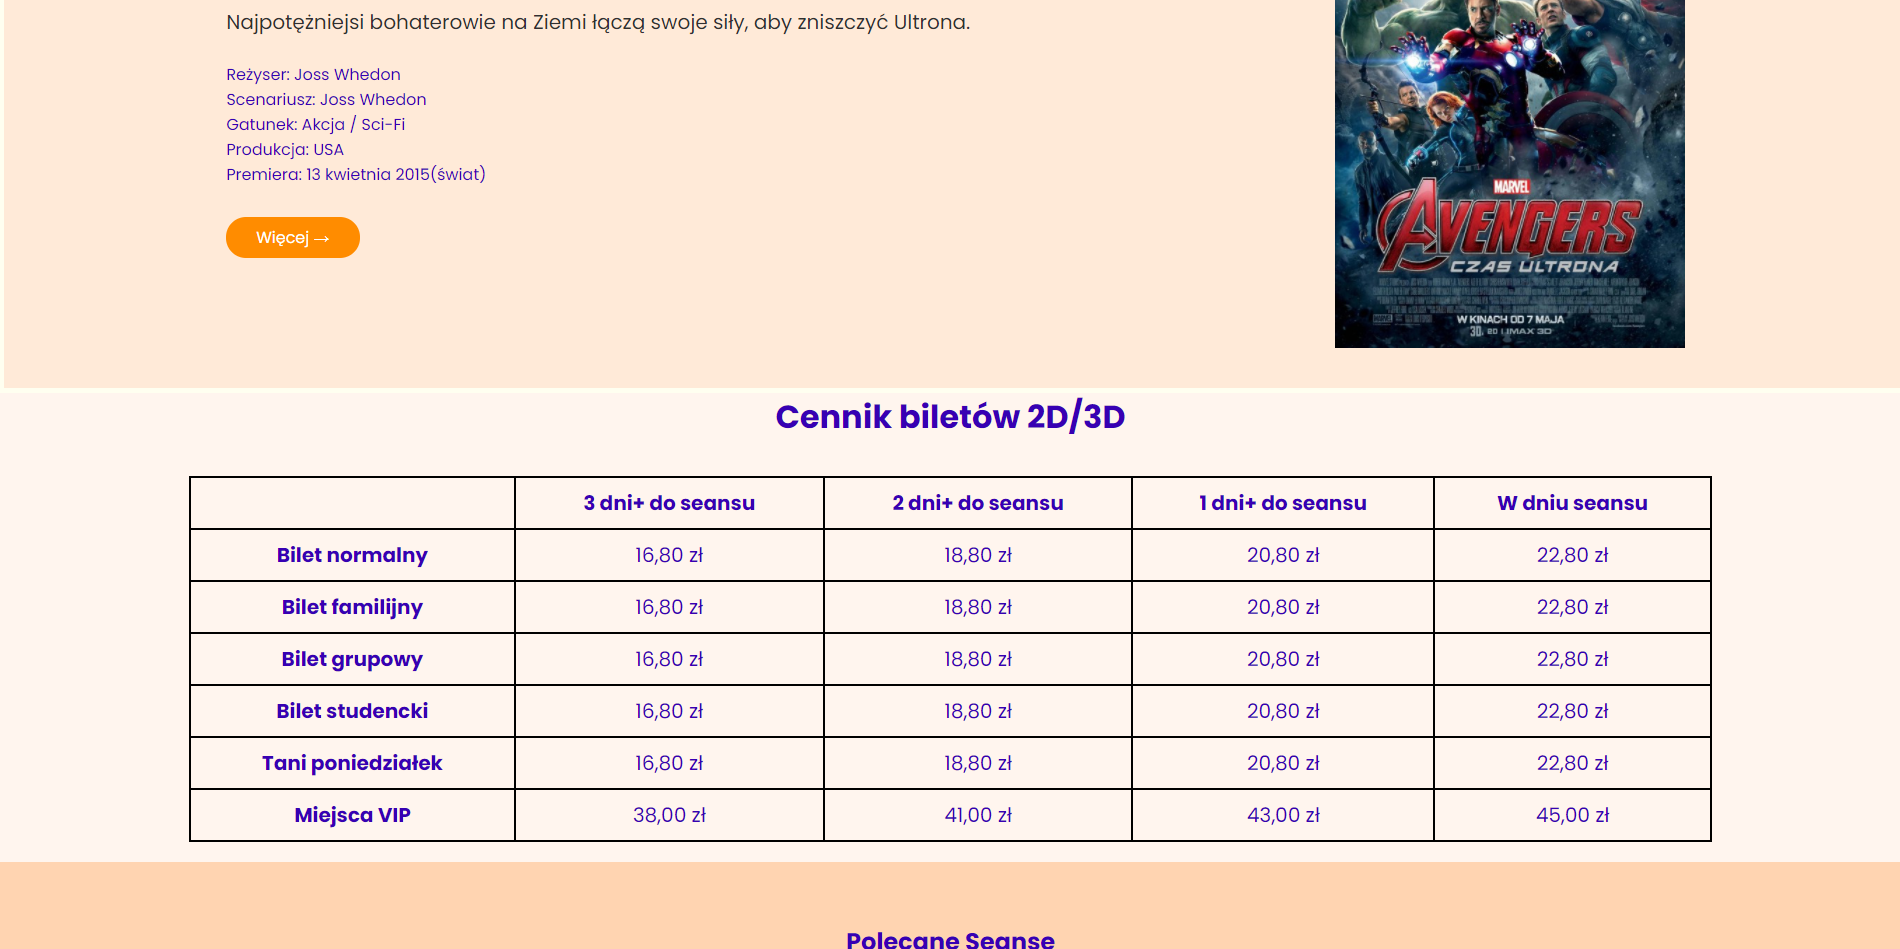
\includegraphics[width=0.9\textwidth]{cennik.png}
  \caption{Cennik.}
\end{figure}
Po wybraniu w menu podstrony "Cennik" klient zostaje przeniesiony do strony z cenami biletów w zależności od spełnionych przez niego warunków (np. bilet ulgowy/normalny).

\newpage
\begin{figure}[h!]
\centering
  \includegraphics[width=0.8\textwidth]{responsywnosc.png}
  \caption{Responsywność strony.}
\end{figure}
Stworzona strona internetowa jest responsywna.



\newpage
\section{Opis usług serwera}
\subsection{Struktura projektu.}
\begin{figure}[h!]
\centering
  \includegraphics[width=0.7\textwidth]{struktura.jpg}
  \caption{Struktura projektu po stronie serwera.}
\end{figure}
W folderze "resources" znajdują się dwa pliki .properties, które odpowiadają dwóm profilom: domyślnemu oraz
developera. Profil domyślny zawiera parametry do połączenia się z bazą danych Postgres w chmurze. Profil developera zawiera parametry do połączenia się z bazą lokalną w celu przeprowadzenia testów.


%%%%%%%%%%%%%%%%%%%%%%%%%%%%%%%%%%%%%%%%%%%%%%%%
\subsubsection{Pakiet "configuration".}
Tabela 1. ukazuje zawartość pakietu "configuration" wraz z opisem klasy.
\begin{table}[H]
\centering
\begin{tabular}{ |p{4.0cm}|p{6.0cm}|  }			

\hline
\textbf{Nazwa klasy lub \textcolor{green}{interfejsu}} & \textbf{Opis klasy}  \\
\hline
CinemaConfig & Klasa konfiguracyjna dodająca filmy do BD przy uruchomieniu serwera. \\
\hline
\end{tabular}
\caption{Pakiet "configuration"}
\end{table}

\subsubsection{Pakiet "customer".}
Tabela 2. ukazuje zawartość pakietu "customer" wraz z opisem klasy.

\begin{table}[H]
\centering
\begin{tabular}{ |p{4.0cm}|p{6.0cm}|  }				

\hline
\textbf{Nazwa klasy lub \textcolor{green}{interfejsu}} & \textbf{Opis klasy}   \\
\hline
Customer & W tej klasie znajdują się podstawowe parametry opisujące klienta. \\
\hline
CustomerController & Klasa, której zadaniem jest odbieranie zapytań HTTP i przekierowywanie sterowania do odpowiedniej metody udostępnianej przez Service. \\
\hline
\textcolor{green}{CustomerRepository} & Interfejs korzystający z JPARepository do pobierania danych z bazy danych.\\
\hline
CustomerSerice & Klasa, która zawiera logikę do przetwarzania danych pobranych z bazy danych.\\
\hline
\end{tabular}
\caption{Pakiet "customer"}
\end{table}

\subsubsection{Pakiet "show".}
Tabela 3. ukazuje zawartość pakietu "show" wraz z opisem klasy.
\begin{table}[H]
\centering
\begin{tabular}{ |p{4.0cm}|p{6.0cm}|  }				
\hline
\textbf{Nazwa klasy lub \textcolor{green}{interfejsu}} & \textbf{Opis klasy}   \\
\hline
Show & W tej klasie znajdują się podstawowe parametry opisujące film. \\
\hline
ShowController & Klasa, której zadaniem jest odbieranie zapytań HTTP i przekierowywanie sterowania do odpowiedniej metody udostępnianej przez Service. \\
\hline
\textcolor{green}{ShowRepository} & Interfejs korzystający z JPARepository do pobierania danych z bazy danych.\\
\hline
ShowService & Klasa, która zawiera logikę do przetwarzania danych pobranych z bazy danych.\\
\hline
\end{tabular}
\caption{Pakiet "show"}
\end{table}

\subsubsection{Pakiet "seat".}
Tabela 4. ukazuje zawartość pakietu "seat" wraz z opisem klasy.
\begin{table}[H]
\centering
\begin{tabular}{ |p{6.0cm}|p{6.0cm}|  }			
\hline
\textbf{Nazwa klasy lub \textcolor{green}{interfejsu}} & \textbf{Opis klasy}   \\
\hline
Seat & W tej klasie znajdują sie podstawowe parametry opisujące miejsce w sali kinowej. \\
\hline
\end{tabular}
\caption{Pakiet "seat"}
\end{table}
%%%%%%%%%%%%%%%%%%%%%%%%%%%%%%%%%%

\subsection{Opis klasy z funkconalnościami serwera.}
Poniżej znajduje się lista funkcjonalności serwera wraz z opisem parametrów wejściowych, wyjściowych oraz
sposób jej działania.
\subsubsection{Klasa CustomerController}
\paragraph{bookSeats}

\textbf{Działanie funkcji:} Metoda, która rezerwuje bilet na wybrany seans dla konkretnego klienta.\\
\textbf{Parametry wejściowe:} Customer customer: obiekt klasy Customer. \\
				 String seats: numer miejsca, które zostało zarezerwowane.\\
				Long showId: id seansu, na który klient zarezerwował miejsce.\\
\textbf{Parametry wyjściowe:} -  \\


\subsubsection{Klasa ShowContoller}
\paragraph{addShow}

\textbf{Działanie funkcji:} Metoda, dodająca seans do bazy danych.\\
\textbf{Parametry wejściowe:} Show show: obiekt klasy show. \\
\textbf{Parametry wyjściowe:} -  \\

\paragraph{getShows}

\textbf{Działanie funkcji:} Metoda zwracająca wszystkie seansy z bazy danych.\\
\textbf{Parametry wejściowe:} - \\
\textbf{Parametry wyjściowe:} List$<$Show$>$  \\

\paragraph{getShow}

\textbf{Działanie funkcji:} Metoda pozwalająca sprawdzić ilość miejsc na dany seans.\\
\textbf{Parametry wejściowe:} Long showId: id seansu \\
\textbf{Parametry wyjściowe:} -  \\

\paragraph{getShowInfo}

\textbf{Działanie funkcji:} Metoda pozwalająca sprawdzić informacje na temat danego filmu.\\
\textbf{Parametry wejściowe:} Long showId: id seansu \\
\textbf{Parametry wyjściowe:} List$<$Show$>$ \\
%%%%%%%%%%%%%%%%%%%%%%%%%%%%%%%%%%%%%%%%%%%%%%%
\section{Narzędzia użyte do stworzenia oprogramowania}
W celu przetestowania działania serwera została użyta aplikacja Postman \footnote{Darmowa aplikacja, która pozwala na wykonywanie zapytań oraz przechowywanie ich historii.}. 
\begin{figure}[H] 						
\centering
  \includegraphics[width=0.5\textwidth]{postman.png}
  \caption{Logo aplikacji Postman.}					
\end{figure}
Poniżej znajdują się screeny potwierdzające poprawność połączenia z bazą danych.

\begin{figure}[H] 					
\centering
  \includegraphics[width=1.0\textwidth]{dodaniefilmudoBD.png}
  \caption{Dodanie filmu do bazy danych.}					
\end{figure}

\begin{figure}[H] 						
\centering
  \includegraphics[width=1.0\textwidth]{rezerwacjamiejsca.png}
  \caption{Rezerwacja miejsca.}					
\end{figure}

\begin{figure}[H] 						
\centering
  \includegraphics[width=1.0\textwidth]{wolnemiejscanakonkrfilm.png}
  \caption{Lista wolnych miejsc na konkretny film.}					
\end{figure}

\begin{figure}[H] 					
\centering
  \includegraphics[width=1.0\textwidth]{wszystkiefilmywBD.png}
  \caption{Lista wszystkich filmów zawartych w bazie danych.}					
\end{figure}

\begin{figure}[H] 						
\centering
  \includegraphics[width=1.0\textwidth]{wyswietlenieinfokonkrofilmie.png}
  \caption{Wyświetlenie wszystkich informacji o danym filmie.}					
\end{figure}

\section{Podział pracy}

{
\centering
\begin{tabular}{ |p{2.2cm}|p{2.2cm}|p{2.5cm}| p{2.2cm}|  }				
\hline
\multicolumn{4}{|c|}{\textbf{Podział pracy}} \\
\hline
Mateusz Łątka & Radosław Urban & Eryk Łuszczkiewicz & Katarzyna Łachut \\
\hline
Implementacja aplikacji serwera. & Implementacja aplikacji klienta.  & Poprawa kodu aplikacji serwera. Testowanie aplikacji. & Stworzenie dokumentacji technicznej \LaTeX.  Testowanie aplikacji.\\
\hline
\end{tabular}
}
\\
Każdy członek zespołu miał znaczący wpływ na wygląd aplikacji oraz dokumentacji.

\section{Linki do repozytorium.}
\href{https://bitbucket.org/mlatka9/project_07_howtoexitvim_client/src/master/} {\Large \textbf{\textcolor{blue}{Aplikacja Klienta}}} \\ \\
\href{https://bitbucket.org/mlatka9/project_07_howtoexitvim_server/src/master/} {\Large \textbf{\textcolor{blue}{Aplikacja Serwera}}} \\ \\
\href{https://bitbucket.org/k_lachut/projekt-07-howtoexitvim-latex/src/master/} {\Large \textbf{\textcolor{blue}{ Kod \LaTeX}}} 



\end{document}